\documentclass[conference]{IEEEtran}
\IEEEoverridecommandlockouts
\usepackage{cite}
\usepackage{amsmath,amssymb,amsfonts}
\usepackage{algorithmic}
\usepackage{graphicx}
\usepackage{textcomp}
\usepackage{xcolor}
\usepackage{tabularx}
\usepackage{multirow}
\usepackage{graphics} % for pdf, bitmapped graphics files
\usepackage{subfig}
\usepackage{subcaption}
\usepackage{hyperref}
\usepackage{academicons}
\usepackage{xcolor}
\usepackage{listings}
\def\BibTeX{{\rm B\kern-.05em{\sc i\kern-.025em b}\kern-.08em
		T\kern-.1667em\lower.7ex\hbox{E}\kern-.125emX}}
% Gráficas en MATLAB
\usepackage{tikz, pgfplots}
% Color Enlace
\definecolor{colorEnlace}{RGB}{0, 0, 0}
\hypersetup{
	colorlinks=true,
	linkcolor=colorEnlace,
	citecolor=colorEnlace,
	urlcolor=colorEnlace,
	pdfauthor={Ruth Juana Espino Puma},
	pdftitle={Informe final 6 - Controlador PD Y PID mediante LGR}
}
% Control 
\usepackage{amsmath}
\begin{document}
	
	\title{Experiencia N°6 - Controlador PD - PID mediante LGR}
	
	\author{
		\IEEEauthorblockN{Ruth Juana Espino Puma}
		\IEEEauthorblockA{
			Estudiante de Ingeniería Electrónica \\
			Cusco, Perú \\
			184657@unsaac.edu.pe}
		\and
		\IEEEauthorblockN{Davis Bremdow Salazar Roa}
		\IEEEauthorblockA{
			Estudiante de Ingeniería Electrónica \\
			Cusco, Perú \\
			200353@unsaac.edu.pe
		}
		\and
		\IEEEauthorblockN{Ing. Darcy Arredondo Huarac}
		\IEEEauthorblockA{
			Laboratorio de Control I\\
			Cusco, Perú\\
			diego.arredondo@unsaac.edu.pe}
	}
	\maketitle
	
	\begin{abstract}
		The design of PD and PID controllers using the root locus method is essential for improving the dynamic performance of control systems. This approach allows engineers to visualize how the poles of a system shift in response to variations in controller parameters, ensuring stability and desired transient behaviors such as overshoot, settling time, and steady-state error. The PD controller primarily enhances system speed and stability by introducing a zero, while the PID controller combines proportional, derivative, and integral actions to achieve a balance between stability, speed, and accuracy. Proper design is crucial to meet performance specifications and avoid instability.
	\end{abstract}
	
	\begin{IEEEkeywords}
		PD controller, PID controller, root locus, stability, transient response, overshoot, settling time, steady-state error, system dynamics, control system design.
	\end{IEEEkeywords}
	
	\section{Informe final}
	La modificación en el comportamiento de los sistemas se puede dar de diferentes métodos el más fácil y sencillo es mediante el cambio de un parámetro modificable (normalmente la ganancia), sin embargo esto no es posible en todo los casos por lo que será necesario agregar un controlador y/o compensador cuando las variaciones de ganancia no sean suficientes para adecuar el sistema al comportamiento deseado, esto se define en \cite{ogata2015} el cual fue el punto de partida para el diseño y desarrollo de controladores PD y PID.
	
	\subsection{\textbf{Muestre las graficas obtenidas con el osciloscopio para el caso subamortiguado en lazo cerrado}}
	
	\subsubsection{\textbf{Controlador PD}}
	Resultado experimental del sistema PD implementado
	\begin{figure}[h]
		\centering
		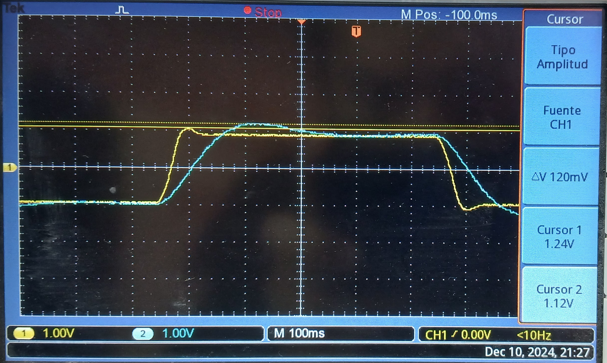
\includegraphics[width=0.5\textwidth]{media/respuesta-sub-implementacion}
		\caption{Respuesta sistema subamortiguado PD - Implementado}
		\label{fig:respuesta-sub-implementacion}
	\end{figure}
	En imagen \ref{fig:respuesta-sub-implementacion} se muestra la respuesta experimental de un sistema controlado mediante un controlador PD para un caso subamortiguado en la cual se observan dos curvas principales, correspondientes a la señal de referencia y la señal de salida del sistema.
	
	\subsubsection{\textbf{Controlador PID}}
	Resultado experimental del sistema PID implementado
	
	\begin{figure}[h]
		\centering
		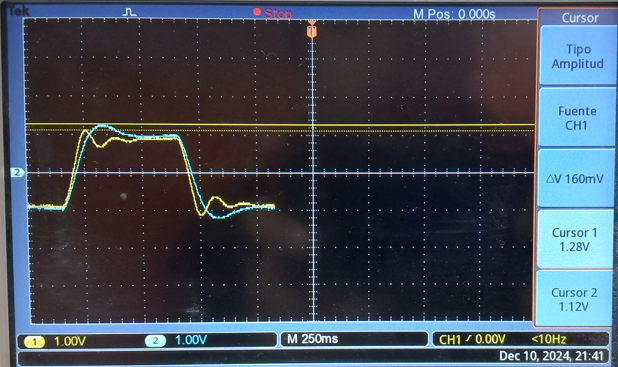
\includegraphics[width=0.5\textwidth]{media/respuesta-sub-pid}
		\caption{Respuesta sistema subamortiguado PID - Implementación}
		\label{fig:respuesta-sub-pid}
	\end{figure}
	En la imagen \ref{fig:respuesta-sub-pid} se presenta la respuesta experimental de un sistema con un controlador PID en condiciones similares de subamortiguamiento en lazo cerrado y en la cual también se tiene una señal de referencia y de salida. La respuesta muestra una mejor convergencia hacia el valor deseado con menor oscilación en comparación con el controlador PD, destacando la capacidad del controlador PID para combinar estabilidad, precisión y velocidad de respuesta mediante sus acciones proporcional, integral y derivativa.
	
	\subsection{\textbf{Analice el error en estado estacionario en el caso subamortiguado con un controlador PD y con un controlador PID en lazo cerrado.}}
	
	El error en estado estacionario es la diferencia persistente entre la salida deseada y la salida real de un sistema de control cuando este alcanza un régimen permanente, es decir, después de que han transcurrido todos los efectos transitorios, el error en estado estacionario depende de las características del sistema, el tipo de entrada aplicada (escalón, rampa, etc.), además reducir este error es crucial para lograr un desempeño preciso en sistemas de control y/o en su defecto poder contar con un valor y tiempo de establecimiento del sistema.
	
	El error en estado estacionario matemáticamente este se define en \ref{eq:ess-posicion-limite} o \ref{eq:ess-velocidad-limite} siendo la diferencia entre ambas ecuaciones el tipo de sistema a analizar, siendo el PID un sistema de tipo 1 y el controlador PD de tipo cero, siendo ello de tal forma a causa de la existencia o no del polo en origen.
	\begin{equation}
		K_p = \lim_{s \to 0} G_c G(s)
		\label{eq:ess-posicion-limite}
	\end{equation}
	
	\begin{equation}
		K_v = \lim_{s \to 0} sG_c G(s)
		\label{eq:ess-velocidad-limite}
	\end{equation}
	
	Para el caso del sistema PD será necesario el calculo de la constante de posición y para el PID la constante de velocidad, siendo así que esta variación también afecta el calculo de la error en estado estacionario para cada caso, como se define en \ref{eq:ess-posicion} esta se usa para un error de posición y \ref{eq:ess-velocidad} para un error de velocidad.
	
	\begin{align}
		e_{ss} &= \frac{1}{1 + K_p} \\
		\label{eq:ess-posicion}
		e_{ss} &= \frac{1}{K_v} \\
		\label{eq:ess-velocidad}
	\end{align}
	
	\subsubsection{Controlador PD}
	\begin{align}
		K_p &= \frac{20(0.026706)(70.5094)(325)}{325} \\
		K_p &= 173.58 \\
		e_{ss} &= 0.00573
	\end{align}
	\subsubsection{Controlador PID}
	\begin{align}
		K_v &= \frac{0.66(0.0049693)(10)(382.3934)(325)}{325} \\
		K_v &= 12.54 \\
		e_{ss} &= 0.07974
	\end{align}

	\subsection{\textbf{¿La respuesta hallada en forma teórica es igual o similar al circuito implementado?}}
	
	Al realizar las comparaciones entre las respuestas para cada sistema entre los valores teóricos, simulados y experimentales se puede apreciar ciertas diferencias no significativas respecto a parámetros como el error en estado estacionario o la respuesta del sistema en régimen transitorio, sin embargo al sintonizar el controlador mediante la ganancia proporcional para cada caso se obtuvo crecientes diferencias respecto a la teoría, no obstante por otro lado se puede notar una pariedad entre los resultados simulados e implementados para pequeñas variaciones en la ganancia.
	
	Las variaciones entre mediciones se puede justificar debido al movimiento de los polos deseados en el lugar de las raíces y la sensibilidad del mismo al modificar la ganancia proporcional, alterado el comportamiento del mismo.
	
	\section{conclusiones}
	\begin{itemize}
		\item El controlador PID muestra una mejor capacidad para reducir las oscilaciones y alcanzar el valor deseado de forma más rápida y precisa en comparación con el controlador PD, destacando su ventaja en sistemas donde la estabilidad y precisión son cruciales.
		\item En el caso del controlador PD, se observa un comportamiento oscilatorio más pronunciado, indicando que este tipo de control prioriza la velocidad sobre la estabilidad. Por otro lado, el controlador PID logra un equilibrio entre ambos factores, mejorando la suavidad de la respuesta transitoria
		\item  Las diferencias observadas entre las respuestas experimentales subrayan la importancia de seleccionar adecuadamente el tipo de controlador en función de los requisitos del sistema, considerando factores como la exactitud, la estabilidad y las condiciones del entorno operativo.
	\end{itemize}
	
	\bibliographystyle{IEEEtran}
	\bibliography{biblio}
\end{document}